

\section{A dynamical model for the emergence of gamete asymmetry}


\begin{figure}[htb!]
    \centering
    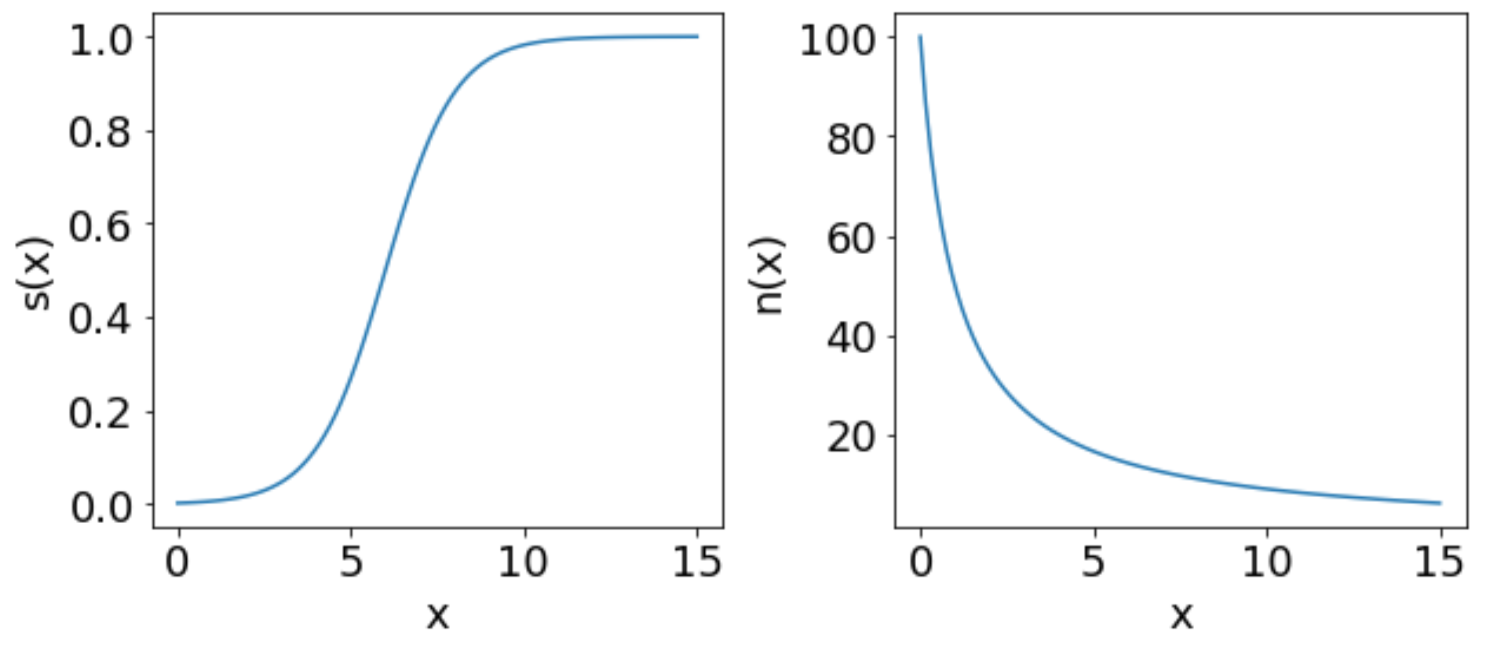
\includegraphics[width = 0.8\textwidth]{vickysFigs/2_sex_funForm}
    \caption{The functional forms of $s(x)$ (left) and $n(x)$ (right), for the parameters in the simulation that generated results in Fig~\ref{fig:2sexRun1}.}
    \label{fig:2sexFun1}
\end{figure}

\begin{figure}[htb!]
    \centering
    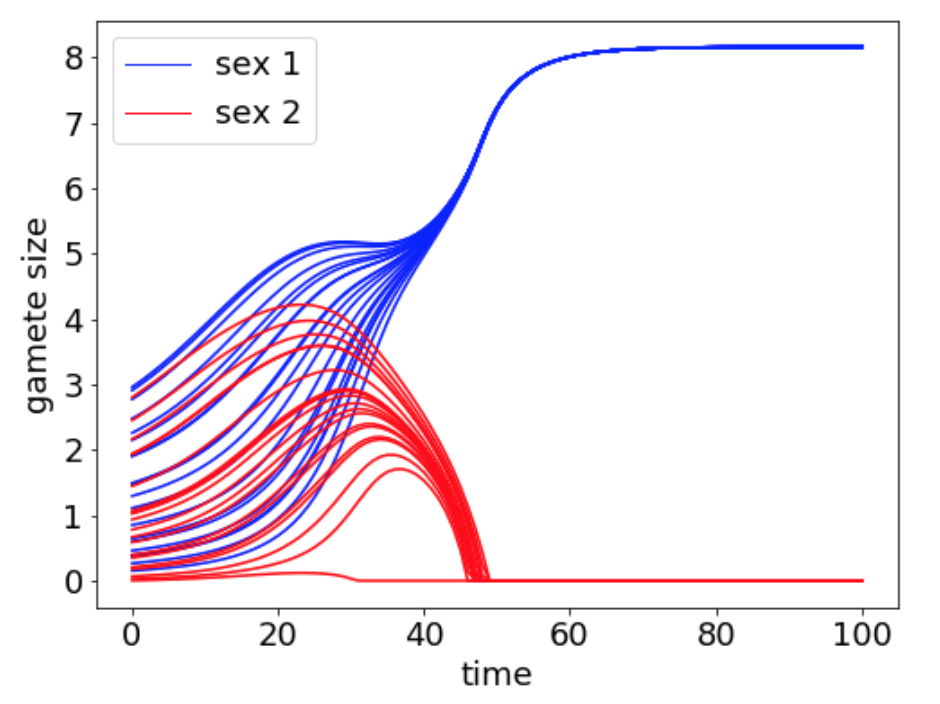
\includegraphics[width = 0.6\textwidth]{vickysFigs/2_sex_run1}
    \caption{Simulation for the gamete size evolution in the case of two sexes. Each curve indicates the evolution trajectory of one initial condition in gamete size. The two colors distinguish gametes of the two sexes. One sex evolves to have the minimal gametes size ($0$), and the other sex evolves to have a large gamete size.}
    \label{fig:2sexRun1}
\end{figure}

In our three-sex world, we have one sex with large gametes (like egg in humans) and two sexes with minimally small gametes (like sperms in humans). To give you humans a more intuitive picture of what the three-sex world looks like, we present here a dynamical model and show, in simulation, show how the Gamete size distribution evolves to be the way it is. 

\subsection{Two sexes}
To convince you of the model's validity, we first present the model in the case of two sexes and show how the model predicts the emergence of gamete size differences on Earth. 

In the model, we use subscript $1$ to denote variables for sex $1$, and subscript $2$ to denote those for sex $2$. Let $x$ denote gamete size (biomass), and $\rho_1(x_1)$ denote the distribution of gamete size in sex 1, and $\rho_2(x_2)$ denote that in sex 2. Let there be $N$ individuals in either sex. We denote the gamete size of all individuals in sex 1 to be $X_1 = (x_{1,1}, x_{1,2}, \cdots x_{1,N})$. We denote that for sex 2 to be $X_2$. 

We denote the minimum size of the gamete to be $x = 0$. Denote the number of gametes an individual produces in one mating event to be $n$, which is expected to decrease with $x$. One function that satisfies this relationship is $n(x) = n_{max}/(x + 1)$, where $n_{Max}$ is the maximum number of gametes possible produced in a mating event, when gametes are at its minimal size. This inverse relationship reflects the conservation of reproductive energy. 
Consider a well-mixed population, where all individuals in sex 1 can mate with all individuals in sex 2, and vice versa. Consider one mating event, where individual of sex 1, with gamete size $x_1$, mate with an individual of sex 2, with gamete size $x_2$. Note that $x_2$ also mates with all other individuals in sex 1 at other times. Then the probability that one of the $x_1$'s gamete merge with the $x_2$ gamete is, $ \frac{n_1(x_1)}{\sum_{x_1\in X_1} n_1(x_1)}S(x_1+ x_2)$. Given that the two gametes merge, in order to produce children successfully, the two merged gametes need to provide enough support in terms of biomaterial. The probability of children's birth success increases with the biomass of the sum of the two merged, with a function we call $S(x_1 + x_2)$. One choice of the function $S$ is the Sigmoid function, $S(x) = 1/(1 + \exp(-k (x - b)))$. 

In this mating event, the number of expected children is the product of the two terms,  

\begin{equation}\label{eq:c1}
    c(x_1, x_2) = \frac{n_1(x_1)}{\sum_{x_1\in X_1} n_1(x_1)}S(x_1+ x_2)
\end{equation}
Integrate over all $x_2$'s, the expected number of total children for an individual of gamete size $x_1$ and sex 1 in all mating events is, 
\begin{equation}
    c_1(x_1) = \sum_{x_2 \in X_2} \frac{n_1(x_1)}{\sum_{x_1\in X_1} n_1(x_1)} S(x_1+ x_2) 
\end{equation}

Similarly, we can write down the number of expected total children for an individual of sex 2, with gamete size $x_2$, 
\begin{equation}
    c_2(x_2) = \sum_{x_1 \in X_1} \frac{n_2(x_2)}{\sum_{x_2\in X_2} n_2(x_2)} S(x_1+ x_2) 
\end{equation}

We assume, over evolutionary time, individuals of both sexes evolve to increase the number of total expected children. we obtain a system of coupled ordinary differential equations (ODEs)

\begin{equation} \label{eq:2sexDynam}
\Bigg\{
\begin{array}{ll}
\frac{dx_1}{dt} = \frac{dc_1}{dx_1} \\
\frac{dx_2}{dt} = \frac{dc_2}{dx_2}  
     \end{array}
\end{equation}
The intuitive understanding of Eq.~\ref{eq:2sexDynam} is that gamete size evolves to the direction that increases the expected number of children for individuals with that gamete size. Note that the collection $X_{1,2}$ changes over time. 

We numerically simulate the model (Eq.~\ref{eq:2sexDynam}) described above in an agent-based fashion, with discrete time steps. We start with 20 individuals in each sex with gamete size drawn from a uniform distribution. The functional form of  $s(x)$ and $n(x)$ with our chosen parameters are shown in Fig.~\ref{fig:2sexFun1}. The trajectories for the evolution of gamete size are shown in Fig.~\ref{fig:2sexRun1}. One sex evolves to have the smallest possible gametes size, and the other evolves to have a large gamete size, agreeing with what we observe on earth. 


\subsection{Three sexes}


\begin{figure}[htb!]
    \centering
    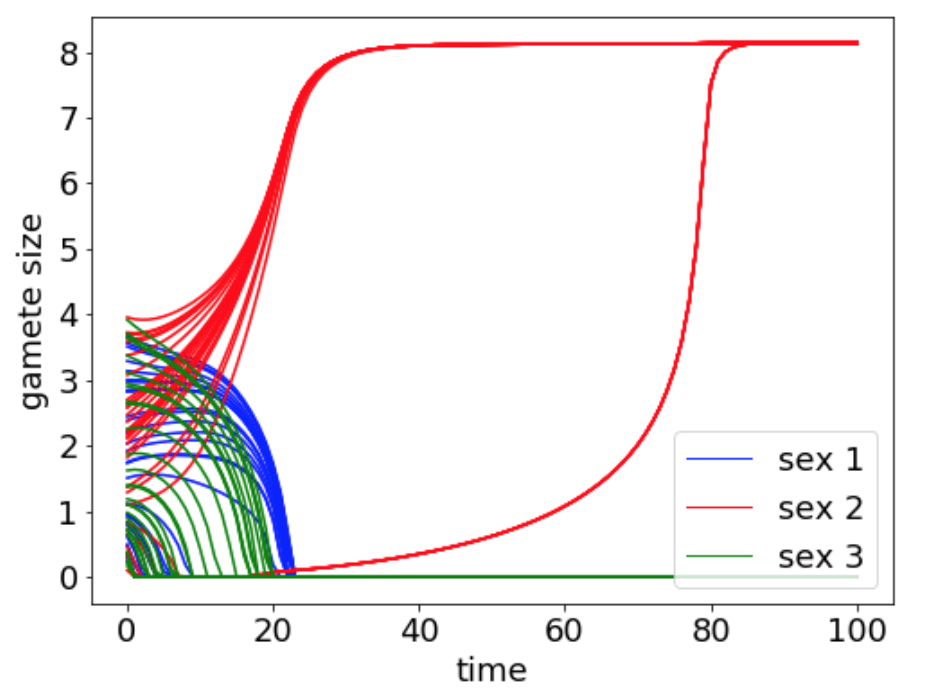
\includegraphics[width = 0.6\textwidth]{vickysFigs/3_sex_run1}
    \caption{Simulation for the gamete size evolution in the case of three sexes. One sex evolves to have a large gamete size and two evolves to have the minimal gamete size. }
    \label{fig:3sexRun1}
\end{figure}


Now we have confidence that the model predicts what happens on Earth, let's take a look at what the models show in the case of three sexes (1, 2, and 3). 

In the world of three sexes, the number of children expected in an mating event with gamete sizes $x_1$, $x_2$, and $x_3$ (similar to Eq.~\ref{eq:c1}) is modified to be
\begin{equation}\label{eq:c3_1}
    c(x_1, x_2, x_3) = \frac{n_1(x_1)}{\sum_{x_1\in X_1} n_1(x_1)} S(x_1+ x_2 + x_3)
\end{equation}
Now we need to integrate $c$ over all mates in sex 2 and sex 3. The expected total number of children for an individual of sex 1 and gamete size $x_1$ is
\begin{equation} \label{eq:c3_2}
    c_1(x_1) = \sum_{x_2 \in X_1} \sum_{x_3 \in X_3}
   \frac{n_1(x_1)}{\sum_{x_1\in X_1} n_1(x_1)} S(x_1+ x_2 + x_3) 
\end{equation}
I believe you earth scientists are smart enough to write down expressions for $c_2$ and $c_3$, which are similar to Eq.~\ref{eq:c3_2}. 

Then the three-sex coupled dynamical system is a three-equation coupled ODE system, 


%\begin{equation} \label{eq:3sexDynam}
%\Bigg\{
%\begin{cases}
%\frac{dx_1}{dt} = \frac{dc_1}{dx_1} \\
%\frac{dx_2}{dt} = \frac{dc_2}{dx_2}  \\
%\frac{dx_3}{dt} = \frac{dc_3}{dx_3} \\
%    \end{cases}
%\end{equation}

\begin{equation} \label{eq:3sexDynam}
\Bigg\{
\begin{array}{ll}
\frac{dx_1}{dt} = \frac{dc_1}{dx_1} \\
\frac{dx_2}{dt} = \frac{dc_2}{dx_2}  \\
\frac{dx_3}{dt} = \frac{dc_3}{dx_3} \\
\end{array}
\end{equation}

Numerically simulating Eq.~\ref{eq:2sexDynam} using the same procedure as above (in discrete time step and discrete individuals) gives the evolutionary trajectories shown in Fig.~\ref{fig:3sexRun1}. One sex evolves to have a large gamete size, and two evolve to have the smallest possible gamete size.
